\section{Overview and Motivation}
Not all data people deal with has a ``vector space"
representation. For example, we might only have a similarity matrix,
like the following: 
\begin{center}
  \begin{tabular}{ | l | l | l | l | l |}
    \hline
    & $x_1$ & $x_2$ & $x_3$ & $x_4$\\
    \hline
    $x_1$ & 0 & 1 & 1 & 1 \\ \hline
    $x_2$ & 1 & 0 & 2 & 2 \\ \hline
    $x_3$ & 1 & 2 & 0 & 2 \\ \hline
    $x_4$ & 1 & 2 & 2 & 0 \\ \hline
    \hline
  \end{tabular}
\end{center}

\textbf{Typical goals}:
\begin{itemize}
\item gain better understanding of the relationship among data points.
\item embed the data into a space (typically $\mathbb{R}^d,l_2$) that
  we understand better. We can then apply off-the-shelf
  models/algorithms etc. 
\end{itemize}

\textbf{Dimensionality Reduction}:
\begin{itemize}
\item Reduce ``noise'' (noise is application-specific; whatever you do
  not care about.) 
\item Increase computational efficiency
\end{itemize}

\textbf{Metric Embedding}:
\begin{itemize}
\item Given a metric space $(X,\rho)$, want to "embed" it into a
  "normed" space $\underbrace{(R^d,l_p)}_{l^p_\rho}$. 
\item Computational efficiency
\end{itemize}

The goal for an \emph{embedding} is a function
$f:\mathbf{X}\rightarrow \mathbb{R}^d$, where $\forall u,v \in
\mathbf{X}$, $||f(u)-f(v)||_{l_p^\rho} \approx p(u,v)$. 
The bad news: in general, there are finite metric spaces
$(\mathbf{X},p)$, where $\mathbf{X}$ is a $n$-point metric space, that
cannot be isometrically embedded into $l_2^d$ for any $d$ (in other
word, no embeddings preserve distance exactly). See the following
figure for an example. 
\begin{figure}[h!]
\begin{center}
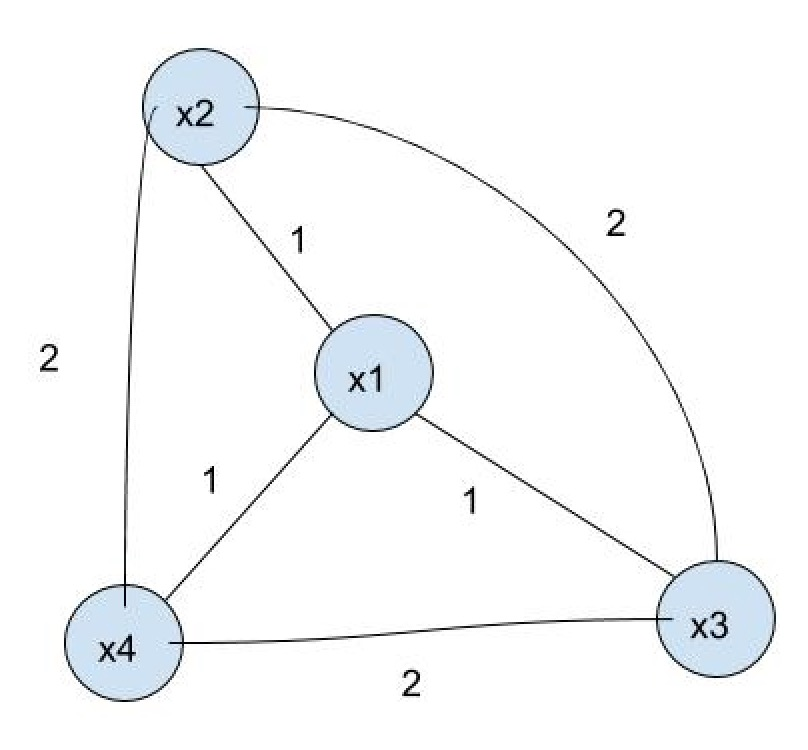
\includegraphics[width=0.5\textwidth]{chapter_5/files/unembeddable.jpg}
\caption{An illustration of not embeddable distance matrix}
\end{center}
\end{figure}

\begin{definition}
Given two metric space $(X,\rho), (Y,\sigma)$. A mapping $f:
X\rightarrow Y$ is called a \emph{$D$-embedding} of $X$ into $Y$
(where $D\geq 1$) if there exists some $r>0$ such that $\forall x,x'
\in X$, 
\[
r \cdot \rho(x,x') \leq \sigma(f(x),f(x')) \leq D \cdot r \cdot
\rho(x,x') 
\]
\end{definition}
